\interlude[3]{Kryptoagilität \\ \hrule \Large \hrule \vspace{1.2em} Leitmotiv}


\SetNextBackground{\includegraphics[width=\paperwidth,page=13]{hpke-slide-designs-2024-05-09}}
\begin{frame}[light]{Fortschritt benötigt fortschrittliche Prozesse}
  \begin{itemize}
    \item Aviate % Handwerkszeug, das eigentliche Tun
    \begin{itemize}
      \item Modularisierung
      \item Continuous Delivery
    \end{itemize}
    \item navigate % Die nächsten Handlungen Planen
    \begin{itemize}
      \item Vorrausplanung
    \end{itemize}
    \item communicate % Zusammenarbeit
    \begin{itemize}
      \item Fordern
      \item Fördern
      \item Zusammenarbeiten
    \end{itemize}
  \end{itemize}
\end{frame}

% \begin{frame}{Schlüssel-Prinzipien}
%   \begin{itemize}
%     \item Proaktives Vorgehen: Kryptoagilität von Anfang an\\
%       $\Rightarrow$ Reaktion muss Vorbereitet sein!
%     \item Modularisierung: Abgrenzungen von Komponenten\\
%       $\Rightarrow$ 
%     \item Regulatorien: Fordern, aber auch Fördern
%     % Regulator: Fördern und Fordern

%     \item aviate navigate communicate
%     \item modularisierung vorausplanen f(ö|o)rdern
%   \end{itemize}
% \end{frame}

% Voerbreiten, hearausfordern, steueen

% TODO drei prinzipien




% \begin{frame}[light]{}
% \begin{itemize}
%   % GOAL Kryptoagilität ist keine Bibliothek die man mitkompiliert, sondern ein komplexer Prozess
%   % GOAL Kontinuierliche Bereitstellung des gesamten Produktes ist teil von den prozes
%   % GOAL Fehlerkultur ist soziale Vorbedingungen für einen Kryptoagilitätsprozess
%   \item Abkehr von der technokratischen Perspektive auf Agilität: Es geht um Prozessgestaltung und soziale Realitäten % Formulierungsidee: Kryptoagilität ist keine Library und auch kein Tool was man installiert. Es ist eine Fähigkeit, die durch umfassende Prozesse Stück für Stück erarbeitet wird.
%   \item Kontinuierliche Bereitstellung: Solange das Produkt eingesetzt wird, ist die Entwicklung nicht beendet
%   \item Fehler akzeptieren – Ein Argument für Bescheidenheit 
%   \item     Planen Sie für Fehlerszenarien, um auf Fehlerszenarien einfach und professionell reagieren zu können
%   \item     Keine Schuldzuweisungen sondern Ursachenfindung für bestmögliche Reaktionen auf Vorfälle
%   \item     Scham und Bestrafung für absichtliches Verschweigen von Problemen
%   \item     Aufbau einer Infrastruktur zur Unterstützung von Einsatzkräften – Serviceorientierung statt Schuldzuweisungen % TODO karo: was sind Einsatzkräft? Meint dies Personal für die Reaktion auf Vorfälle? Dann würde ich vielleicht von Incident Response Teams sprechen.
% \end{itemize}
% \end{frame}
